
\section{Implementación}
En este capítulo expondremos la implementacion tanto del servidor como de la aplicación móvil.


\subsection{Servidor}
En capítulos anteriores ya comentamos la estructura de paquetes seguida para desarrollar el servidor, en este hablaremos de JpaRepository.\\

JpaRepository es un repositorio que nos ofrece métodos genéricos de gestión de clases persistentes como también métodos mas concreto que nos permiten realizar operaciones complejas abstrayendonos de su implementacion.

Ademas este repositorio se adapta a la clase con la que va a trabajar.
\begin{figure}[H]
		\centering
		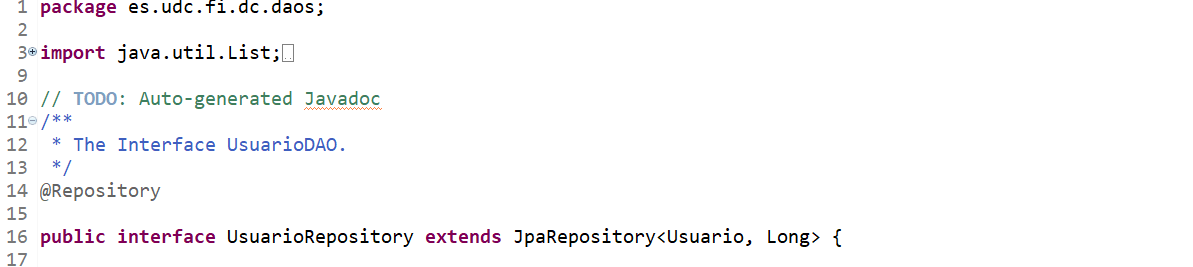
\includegraphics[width=1\textwidth] {jpa.png}
		\caption{UsuarioRepository}
	\end{figure}
	
Como se puede ver en la figura anterior, este interfaz importa la clase Usuario accediendo a todos sus atributos y generando una lista de métodos para estos atributos concretos como podemos ver en la siguiente.
\begin{figure}[H]
		\centering
		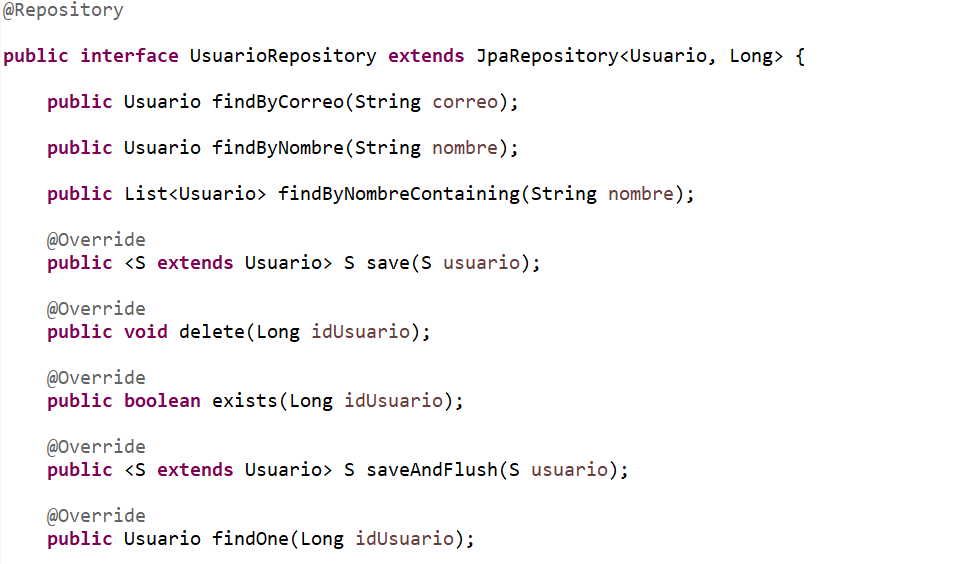
\includegraphics[width=0.5\textwidth] {jpa2.png}
		\caption{UsuarioRepository métodos}
	\end{figure}


\newpage

 
 
 
 
 \subsection{Aplicación móvil Android}
En este capítulo comentaremos aspectos concreto de la implementación de de la aplicación móvil.



\subsubsection{Mapas}

 Para la creación de rutas tanto individuales como compartidas como para crear PDI el usuario necesita conocer las coordenadas de los puntos por lo que trascurre su ruta. Para ello necesitamos los mapas de Google Maps y métodos de sus APIs.
 
\begin{figure}[H]
		\centering
		
\includegraphics[width=0.5\textwidth] {maps.png}
		\caption{Dependencias de mapas para Gradle}
	\end{figure} 
 
 
 Con la dependencia de la figura anterior permitimos a nuestra aplicación que use los servicios de  Google Maps.\\
 Para marcar un punto en el mapa y que este quede visible en el mapa necesitamos implementar un método que capture los clic en el mapa y que nos devuelva las coordenadas del punto marcado.
 
 \begin{figure}[H]
		\centering
		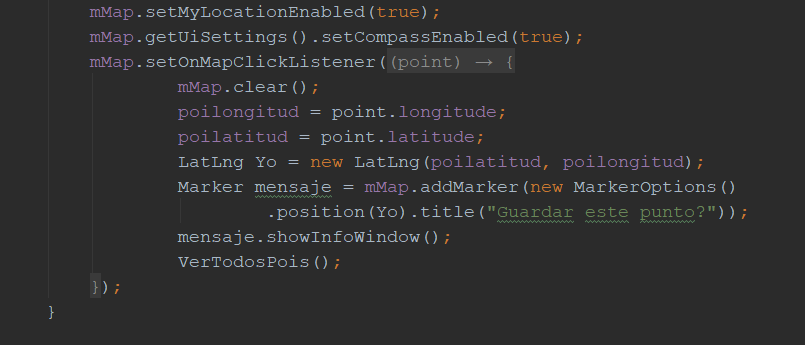
\includegraphics[width=0.75\textwidth] {click.png}
		\caption{Fragmento de código  para capturar el clic}
	\end{figure} 
  Con el fragmento de código de la figura anterior  se capturaría ese clic y aparecería el Marker común de todos los mapas de Google Maps acompañado del mensaje \textit{"Guardar este punto?"}. En nuestro proyecto personalizamos los Marker de modo que cuando guardamos ese punto pase a a representarse con icono de un pescador o de un cazador dependiendo del PDI que estuviéramos guardando. Para ello usamos el siguiente fragmento de código.

 

 \begin{figure}[H]
		\centering
		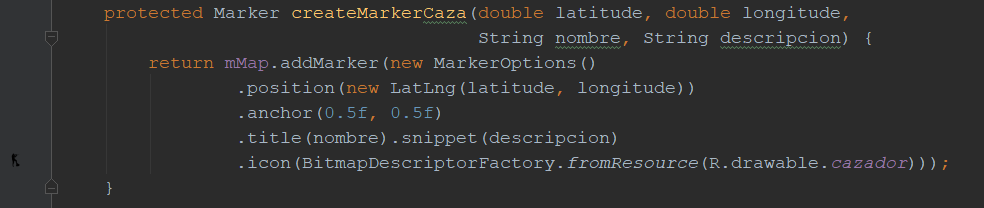
\includegraphics[width=0.75\textwidth] {marker.png}
		\caption{Fragmento de código para la personalización de los Marker}
	\end{figure}
 
 
 
 Y así es como quedaría.  

 
 
 
	\begin{figure}[htbp]
\begin{minipage}[b]{0.5\linewidth} %Una minipágina que cubre la mitad de la página
\centering
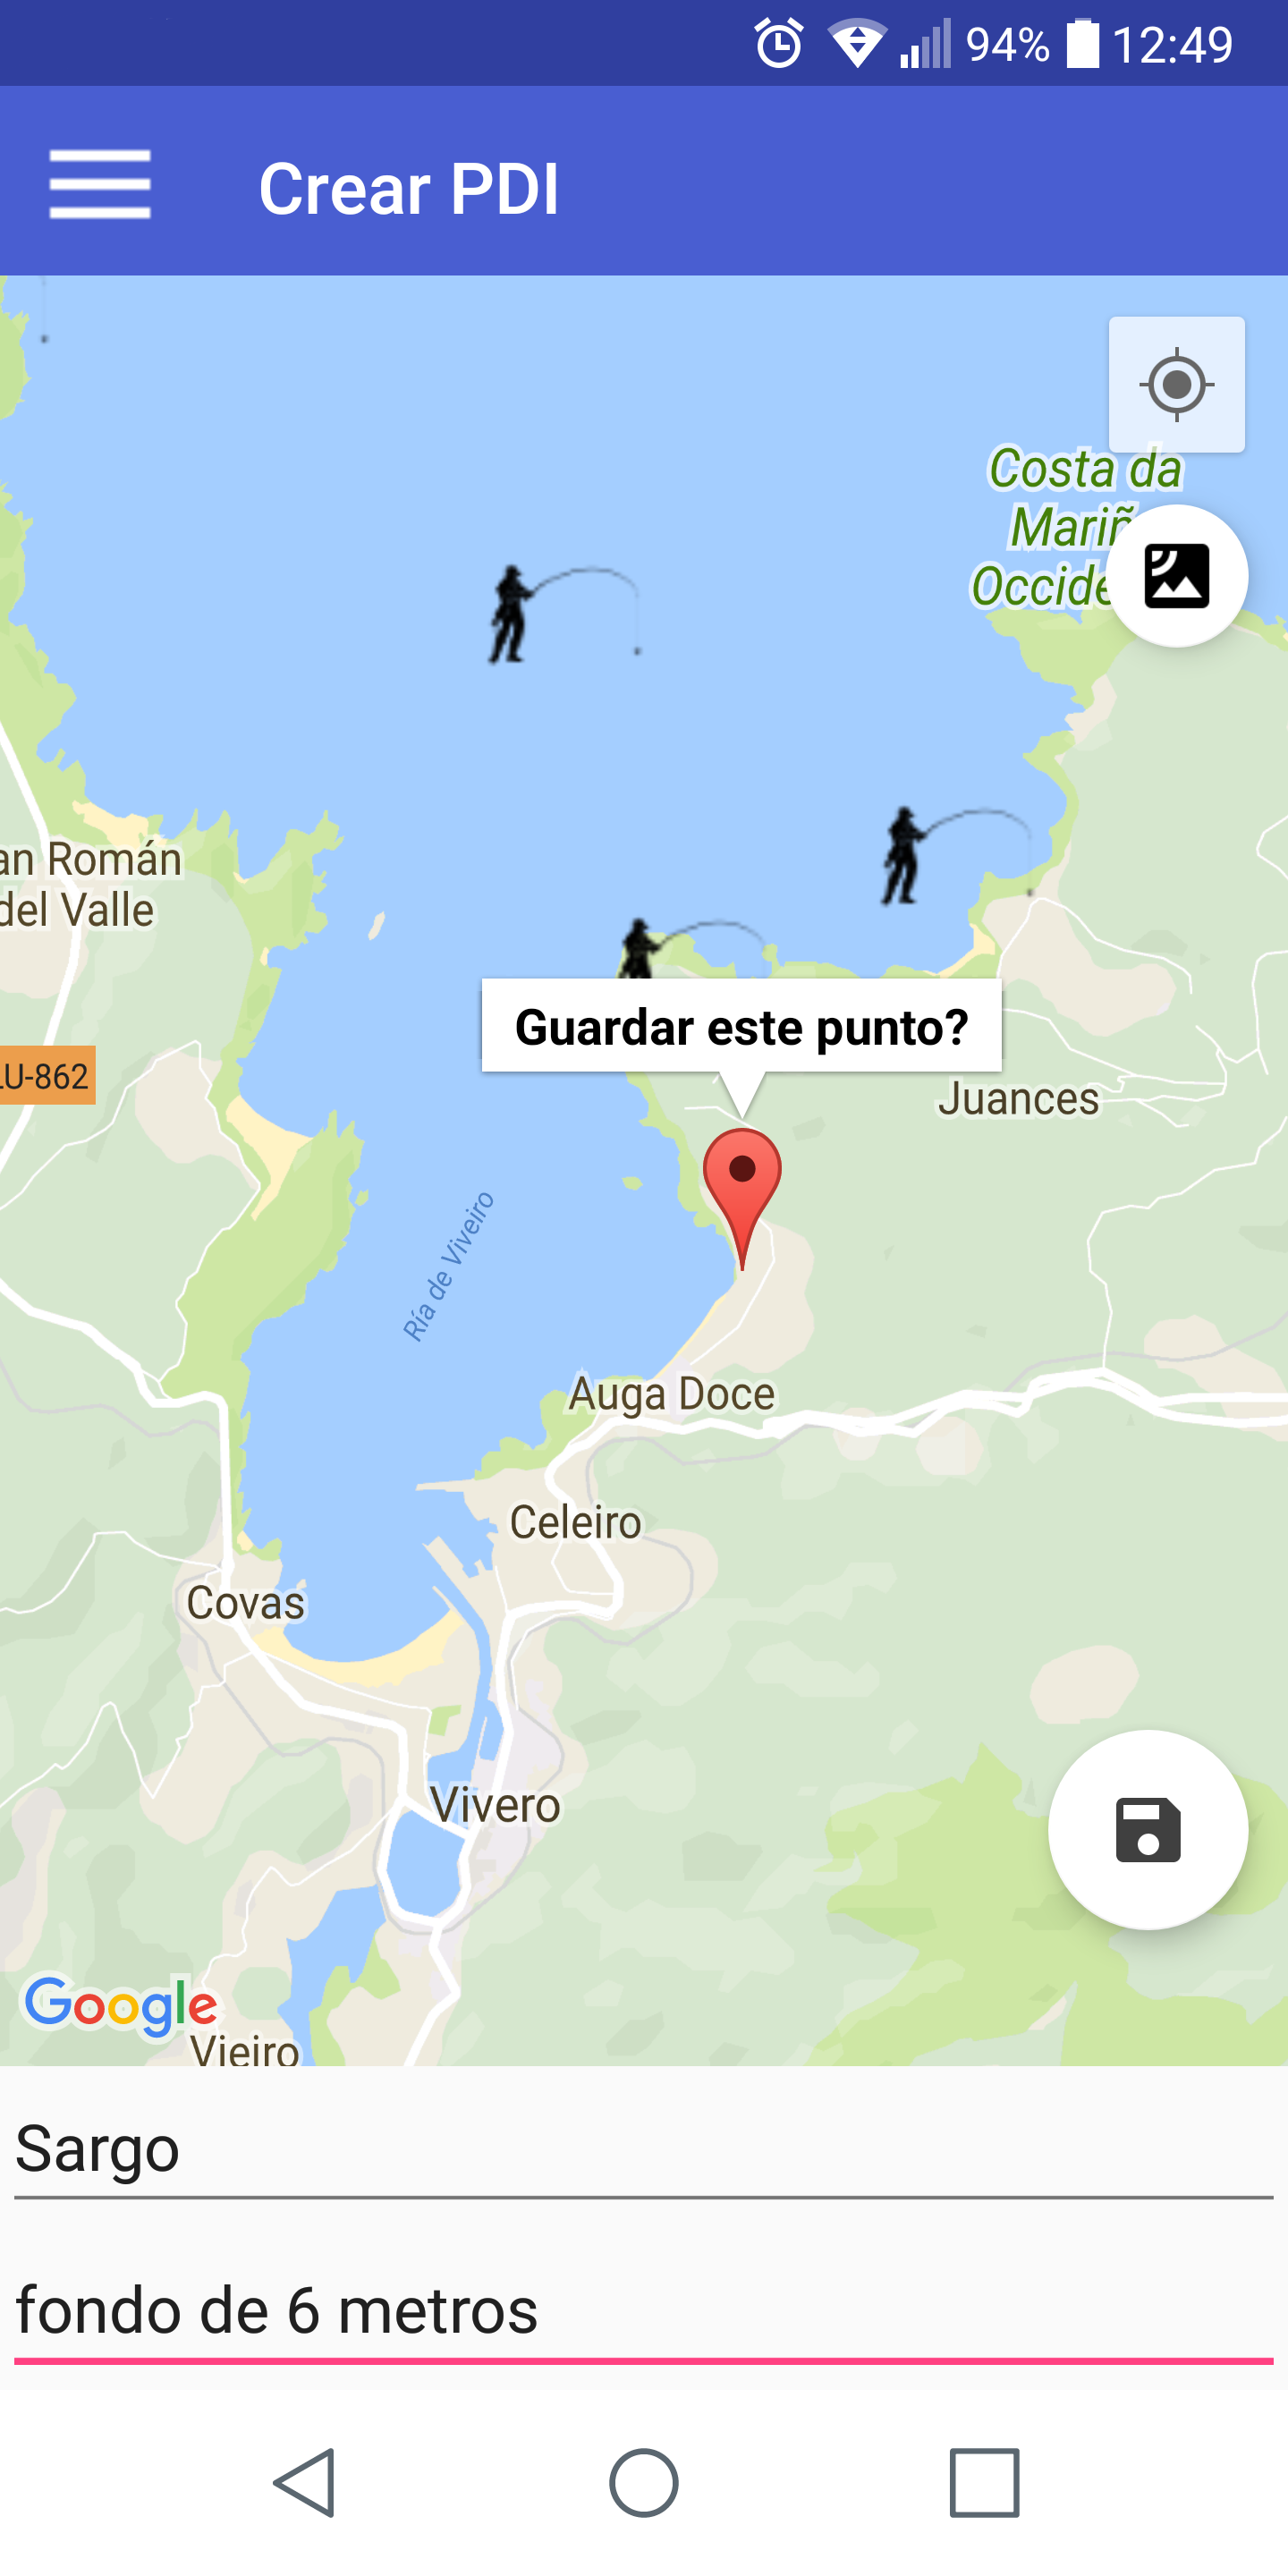
\includegraphics[width=6cm]{capturamovil/pdiguardar.png}
 \label{figura1}
\caption{Marker antes de guardar el PDI}

\end{minipage}
\hspace{0.5cm} % Si queremos tener un poco de espacio entre las dos figuras
\begin{minipage}[b]{0.5\linewidth}
\centering
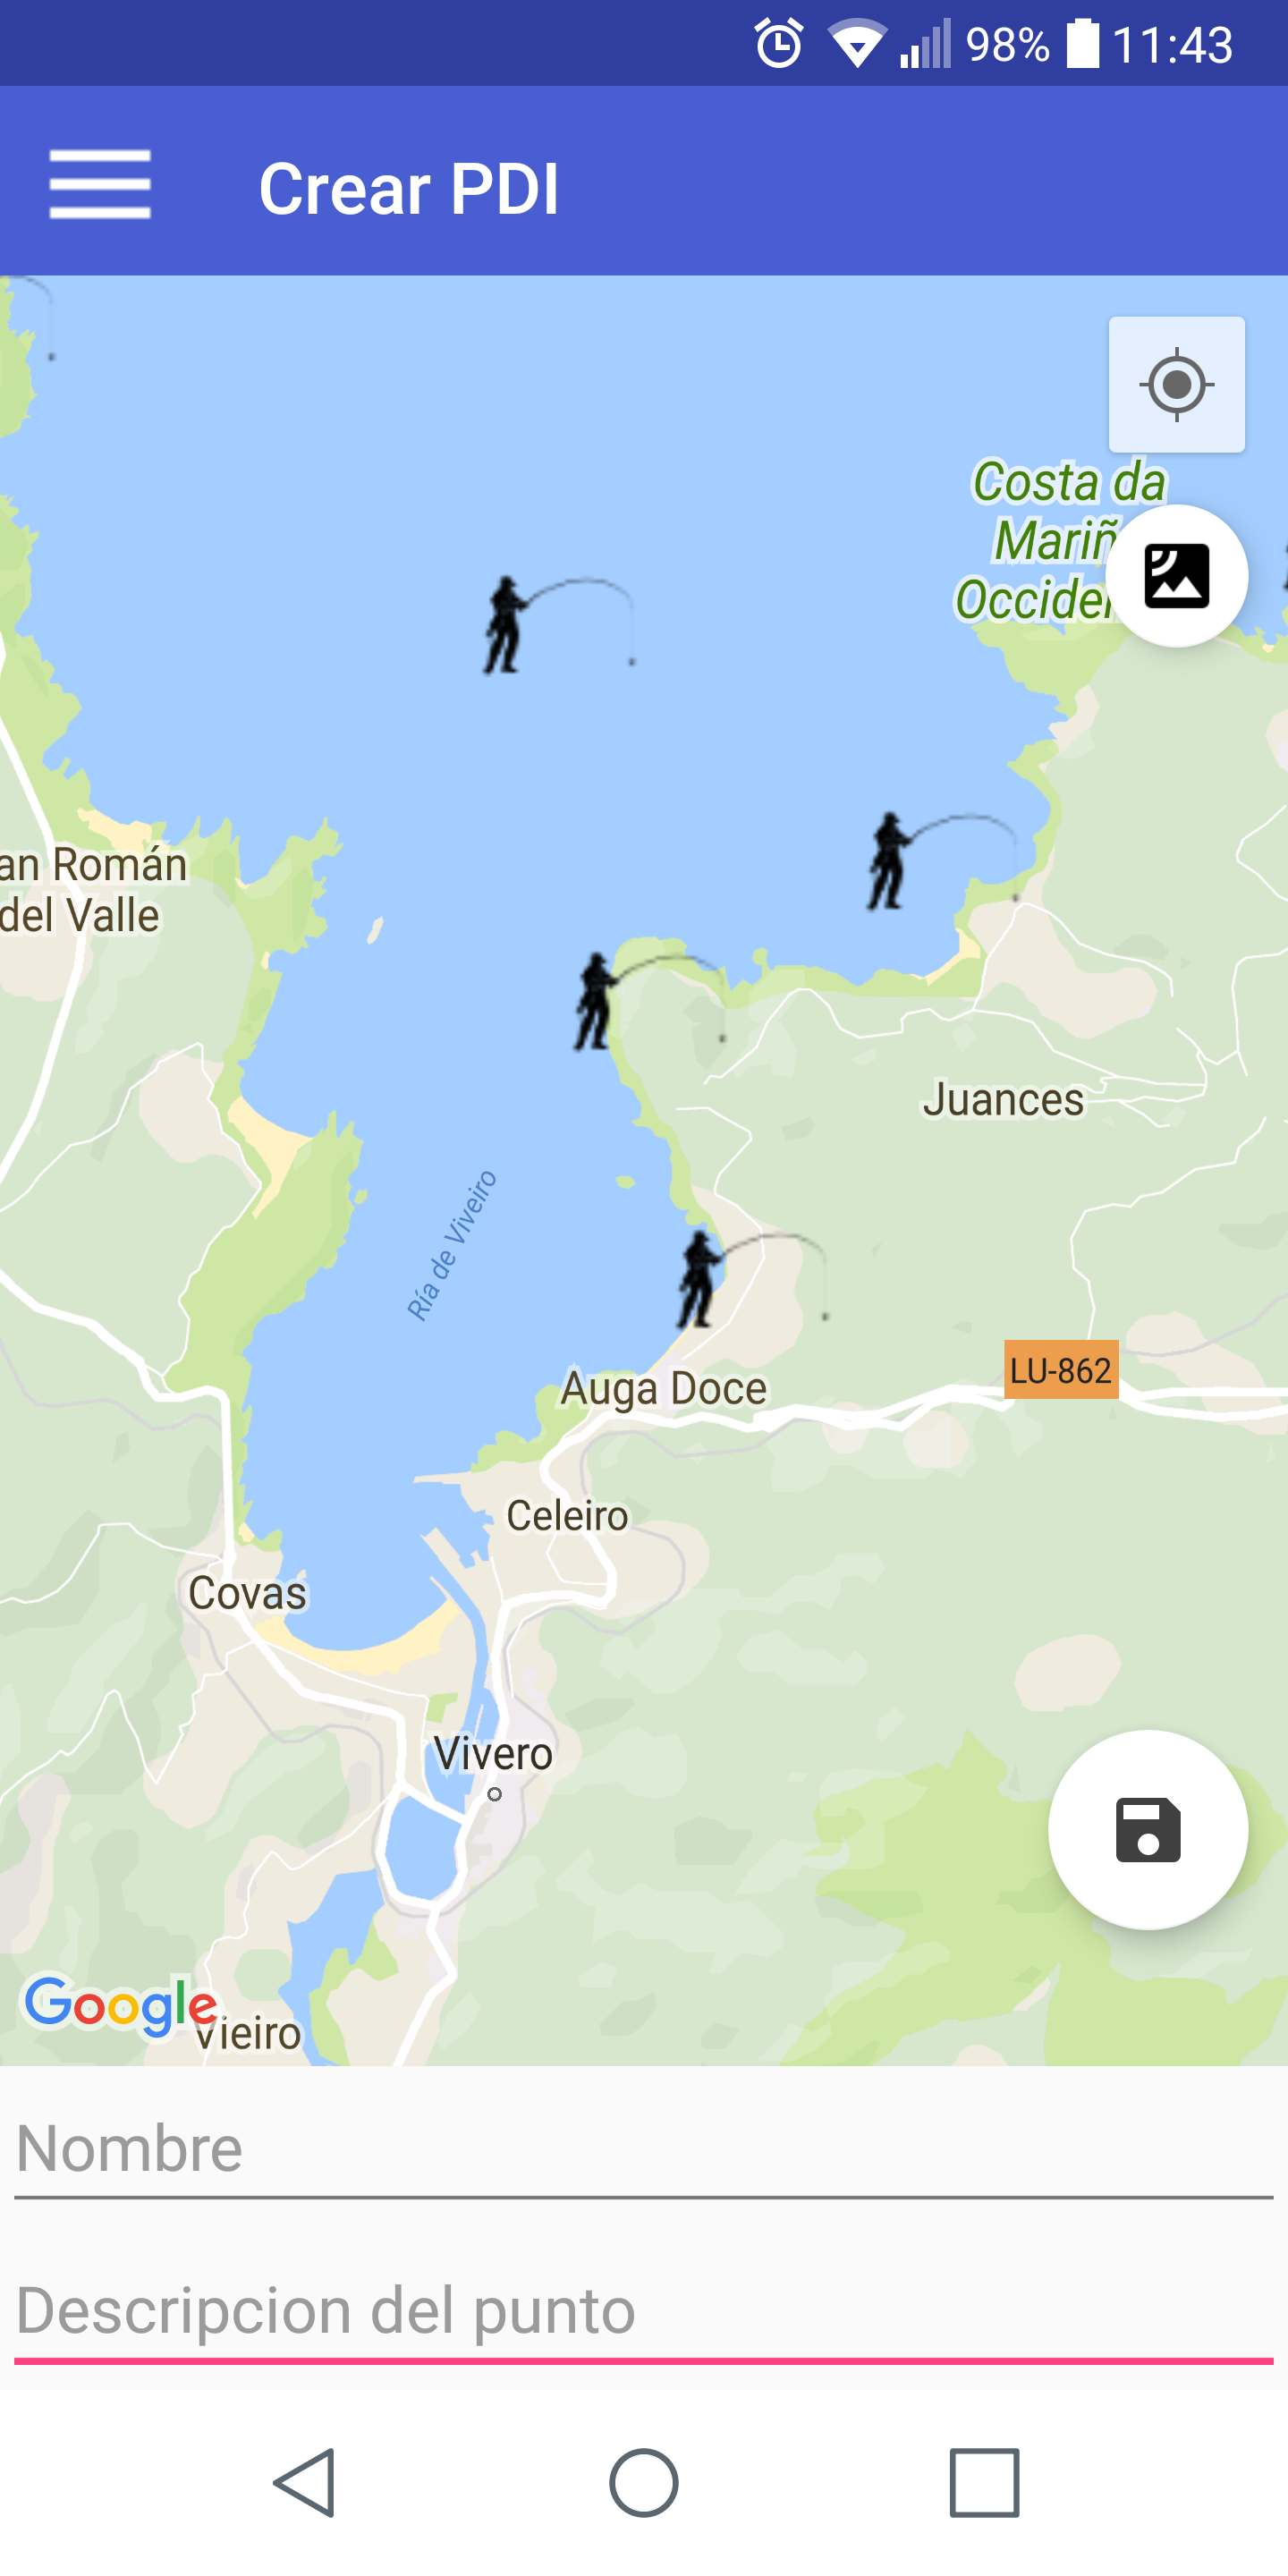
\includegraphics[width=6cm]{capturamovil/pdiguardar2.png}
 \label{figura2}
\caption{Marker después }

\end{minipage}
\end{figure} 
 
 
 
 \subsubsection{Localización}
  Para la creación de ruta necesitamos una método que nos proporcione las coordenadas(latitud y longitud) de los puntos por los que trascurre el usuario en la ruta. Para ellos necesitamos la siguiente dependencia.
\begin{figure}[H]
		\centering
		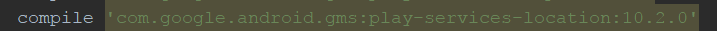
\includegraphics[width=0.5\textwidth] {location.png}
		\caption{Dependencias de gradle para la obtención de la localización}
	\end{figure}
	Una vez añadida esta dependencia necesitamos un método que nos proporciones las coordenadas concretas, para ellos usaremos el siguiente fragmento de código.
	
\begin{figure}[H]
		\centering
		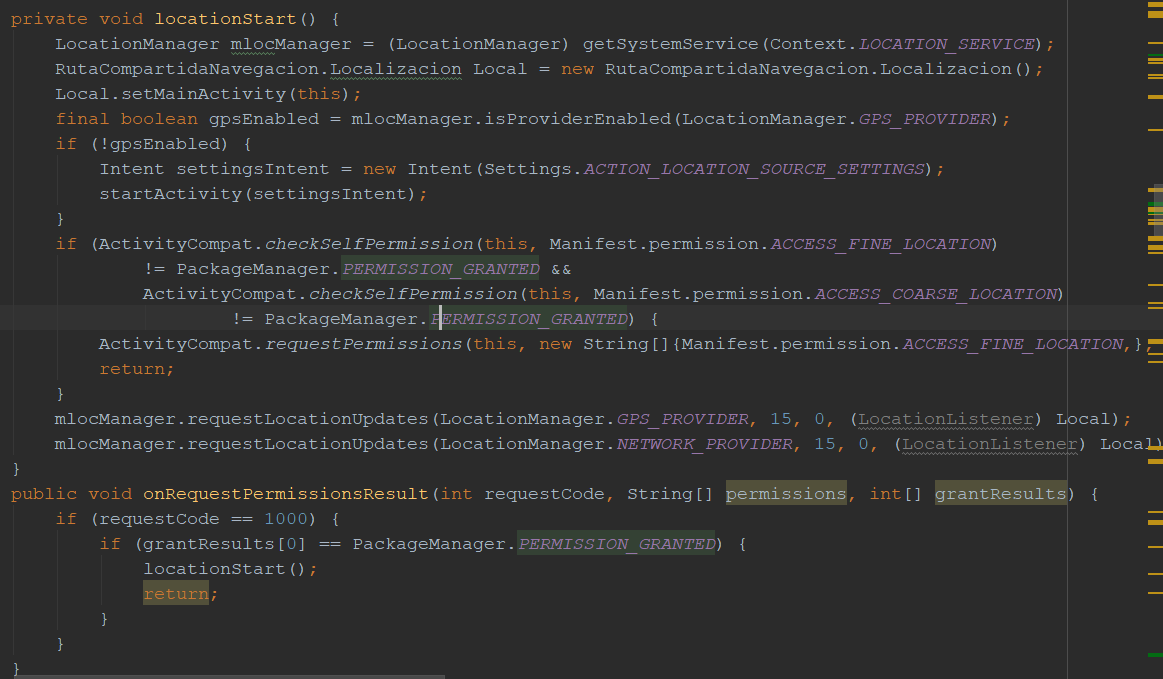
\includegraphics[width=0.75\textwidth] {location2.png}
		\caption{Fragmento de código para obtención de coordenadas}
	\end{figure}

El método ofrece el par de coordenadas cuando el usuario se mueve X metros o bien por un intervalo de tiempo en segundos.

\begin{figure}[H]
		\centering
		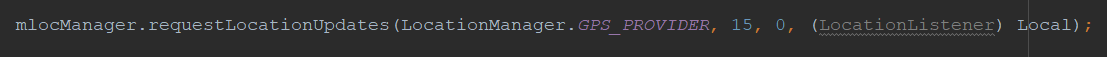
\includegraphics[width=0.75\textwidth] {metros.png}
		\caption{Fragmento de código para obtención de coordenadas}
	\end{figure}

Como se puede observar en la figura anterior en nuestro proyecto indicamos que los segundos que deberían transcurrir para devolver una coordenadas sería de 15.\\
Cuando nosotros estamos realizando la ruta en ocasiones el GPS pierde precisión y sitúa al usuario en punto un tanto lejano, lo cual es imposible ya que no se puede mover tan rápido. Este error del GPS lo hemos resuelto de la siguiente manera.

\begin{figure}[H]
		\centering
		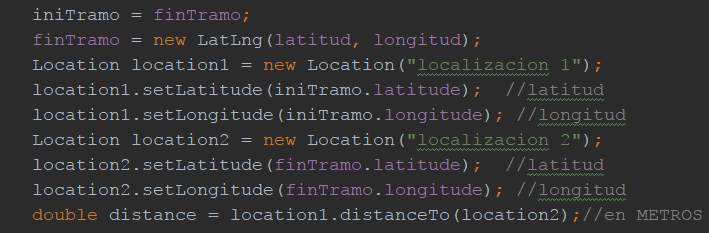
\includegraphics[width=0.75\textwidth] {distancia.png}
		\caption{Código para el cálculo de la desviación de un punto}
	\end{figure}

En este código lo que hacemos es calcular la distancia entre dos puntos consecutivos. Este método pertenece a la API, para calcularla necesita el par de coordenadas y el ya se encarga de tener en cuenta la curvatura de la tierra para hacer la medición. Si esta distancia es superior a 15 metros desechamos ese punto.


	
\subsubsection{Firebase} 
Cuando el usuario inicia una ruta compartida la forma en la que avisa al resto de usuario que la acaba de iniciar es mediante las Notificaciones Push con Firebase. Para ello tenemos que empezar añadiendo las dependencias siguientes.
\begin{figure}[H]
		\centering
		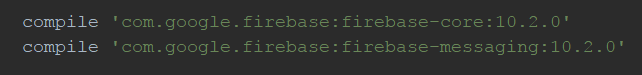
\includegraphics[width=0.5\textwidth] {firebase.png}
		\caption{dependencies Firebase}
	\end{figure}
	
	\begin{figure}[H]
		\centering
		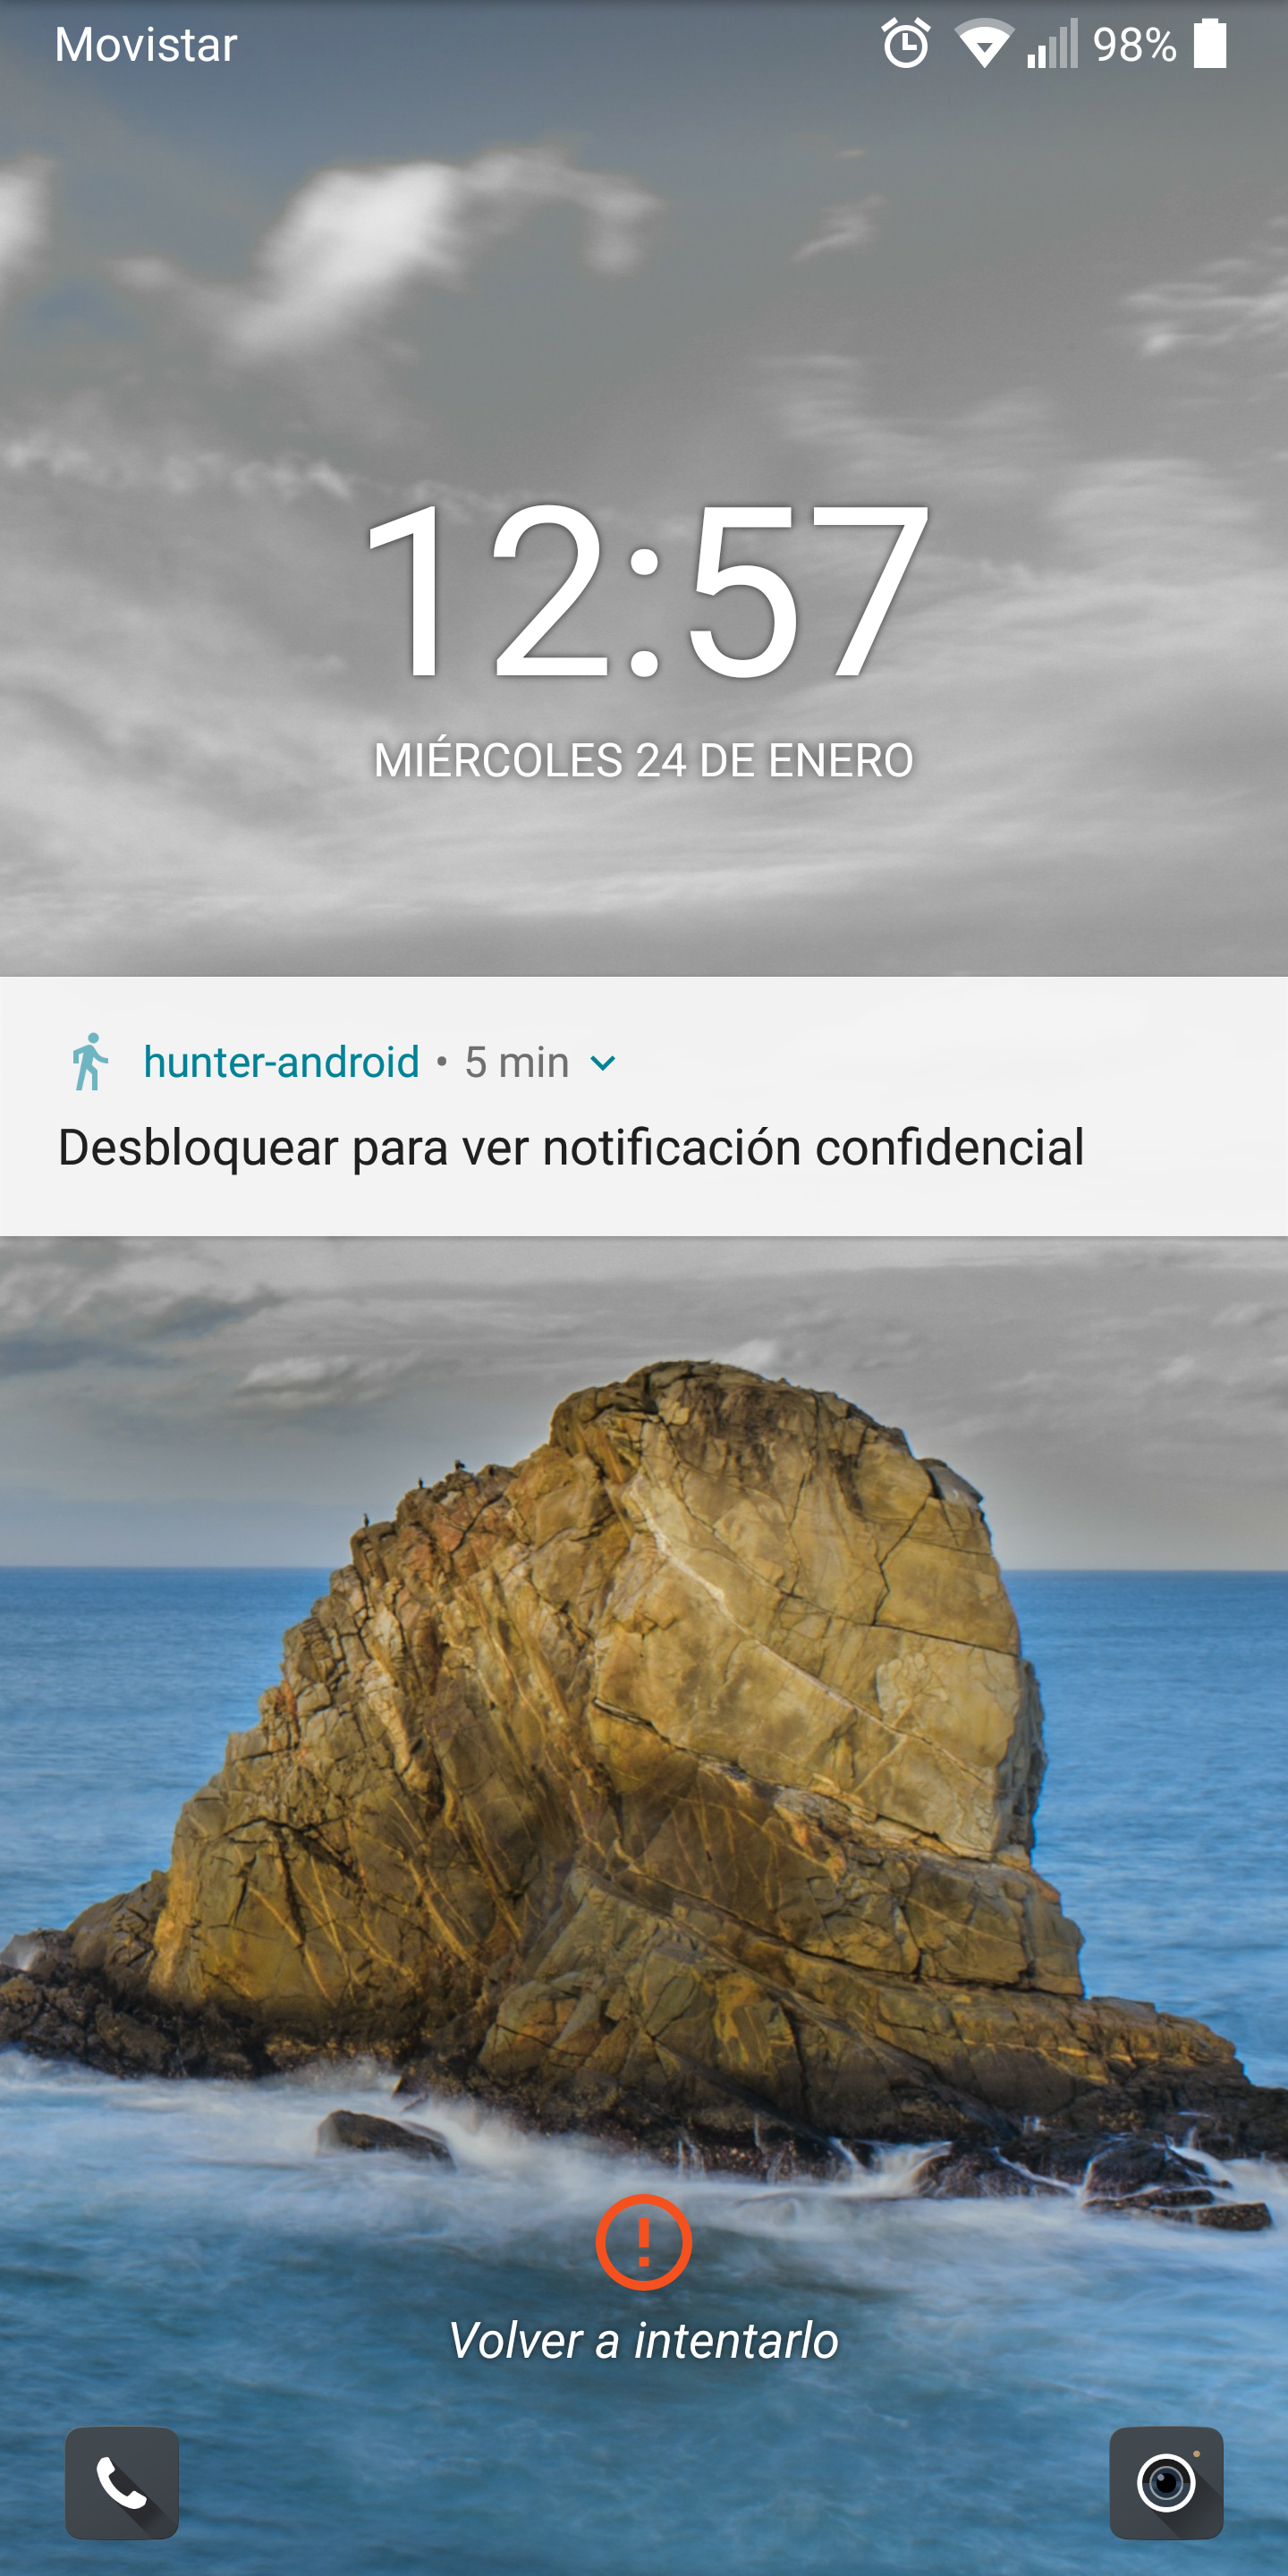
\includegraphics[width=1\textwidth] {push2.png}
		\caption{dependencies Firebase}
	\end{figure}	
\begin{figure}[H]
		\centering
		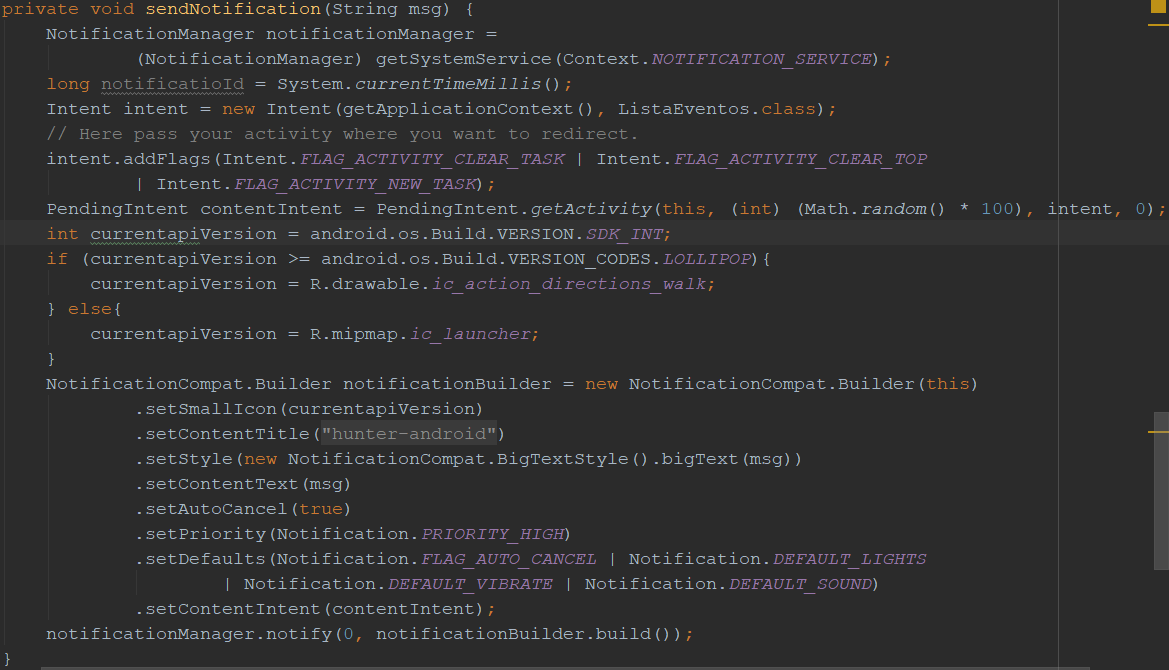
\includegraphics[width=1\textwidth] {push.png}
		\caption{dependencies Firebase}
	\end{figure}	
	
\subsubsection{SQLiteHelper}
\begin{figure}[H]
		\centering
		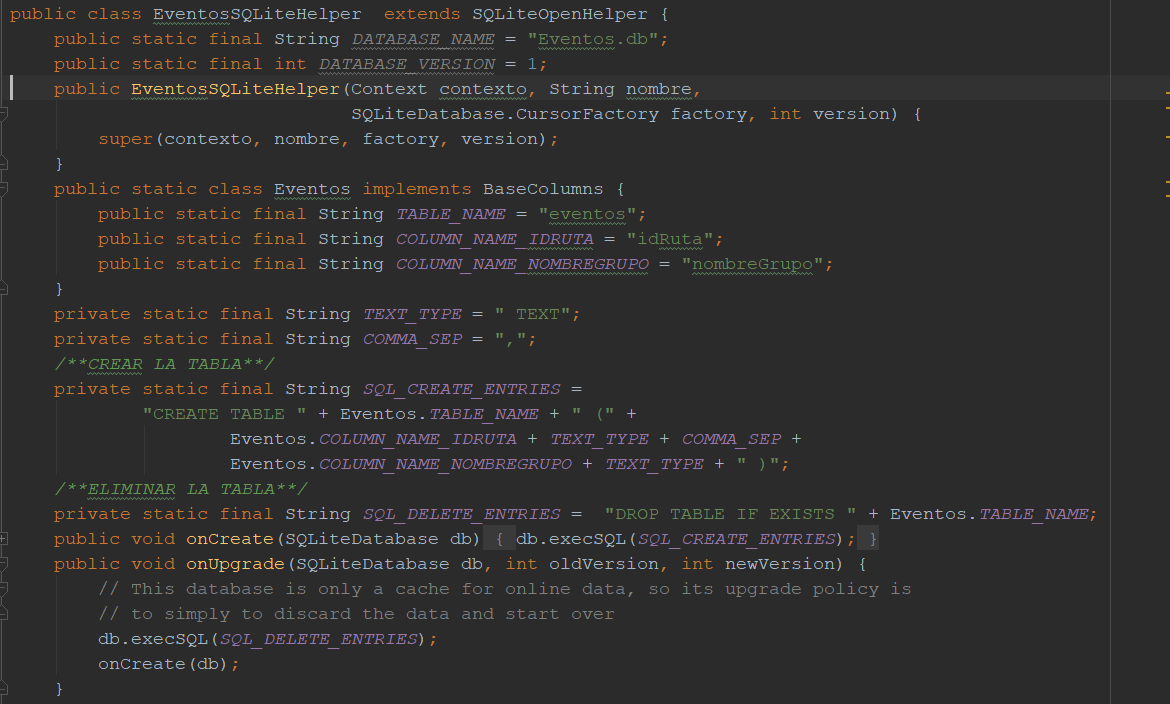
\includegraphics[width=1\textwidth] {sql.png}
		\caption{dependencies Firebase}
	\end{figure}	
	
\section{Pruebas}
\subsection{Pruebas de unidad}
\subsection{Pruebas de unidad y de integración}


